% !TeX root = main.tex
\lecture{4}{Thu 29 Jan 2026 13:00}{Matter IV: Surface Tension and Capiliary Action}

Recap from last time:
\begin{itemize}
    \item Force and potential are related, with $F = \frac{-dV}{dx}$, with $x$ relating to position.
    \item At equilibrium, neighbouring atoms sit at distance $r_0$ (average bond length) from each other. They sit in a potential well of depth $N \epsilon$ where $N$ is the number of nearest neighbours.
    \item At $x < r_0$, the force is +'ve (repulsive), at $x>r_0$ the force is -'ve (attractive).
\end{itemize}

\section{Coordination Numbers}
\begin{figure}[H]
    \centering
    
\includegraphics[width=0.75\textwidth]{figures/lec04-01.png}
     \caption{}
\end{figure}

In a densely-packed Face-Centred Cubic (left) or Hexagonally Close-Packed Solid (3D, middle - 2D, right) configuration, the maximum coordination number (number of nearest neighbours) is $12$. The outermost.

For solids, we expect an interatomic spacing of $\sim 2 \times 10^{-12}$m, for liquids we expect $3 \times 10^{-10}$m and for gases at STP we expect about $40 \times 10^{-10}$m.

For liquids, we expect a coordination number $n<10$.

\section{Molecular/Structural Binding Energies}
To first order (nearest neighbours only), how much energy do we need to remove the innermost atom (orange in the middle figure) from the centre of the structure.

We might expect $12 \epsilon$, the total binding energies of all of the nearest neighbours. Instead however, we are leaving the 12 nearest neighbours in place and only taking one atom to infinity. Since moving both atoms to infinity is given by $\epsilon$, we have:
\[
    E = \frac{n \epsilon}{2}
\]

Where $n$ is the number of nearest neighbours.

To remove one mole of connected atoms, we have:
\[
    E = \frac{n N_A \epsilon}{2}
\]

Again, the factor of two arises to avoid double-counting bonds, i.e. a mole consists of $N_A / 2$ pairs of atoms.


\section{Latent Heat}
Moving macroscopically, we have seen:
\[
    L = 10 \epsilon / 2 \times \frac{\text{number of atoms}}{\text{mass of material, kg}}
\]

For a liquid of coordination number $10$. This is very similar to the just seen:
\[
    E = \frac{n N_A \epsilon}{2}
\]

As $N_A$ gives us atoms per mol, this is effectively identical - one just considers moles and one considers mass in kg.

The molar latent heat equation assume however that the molecular energy comes exclusively from potential energy. This is an approximation that works when kinetic energy is much less than potential energy, i.e. at low temperatures. We can empirically see that molar latent heat varies with temperature:

\begin{figure}[H]
    \centering
    
\includegraphics[width=0.75\textwidth]{figures/lec04-02.png}
     \caption{}
\end{figure}

This is because, at higher temperatures, the average bond length increases (as the particles have a greater kinetic energy, so vibrate with a larger magnitude):

\begin{figure}[H]
    \centering
    
\includegraphics[width=0.75\textwidth]{figures/lec04-03.png}
     \caption{}
\end{figure}

Because the LJP is antisymmetric, at higher temperatures the molecules spend less vibrational time in the contracted position and more time in the expanded position, resulting in a larger average bond length. Effectively, they experience more repulsion when they are together than they do attraction when apart, hence a larger bond length on average. This also explains thermal contraction.

We can see from the potential graph that this results in a lower $\epsilon$, which is why we see a change in latent heat at different temperatures.

\section{Surface Tension}
Consider a (literal) sea of particles. Does a particle surrounded on all sides deep in the liquid experience a lesser or greater potential than a particle on the surface?

The particle deep in the liquid has twice as many nearest neighbours (being surrounded on all sides) so has a greater potential. The particle on the surface will have:
\[
    V = \frac{n \epsilon}{4}
\]

So requires $n \epsilon / 4$ amount of work to take a deeper particle to the surface.

We define a quantity called surface tension $\gamma$, the work done to move $1 \si{m^2}$ of particles, $N$ to the surface from deeper inside the liquid:

\[
    \gamma = \left(\frac{n \epsilon}{2} - \frac{n \epsilon}{4}\right) \times N
\]

Where $N$ is the number of particles per $m^2$. It has units of energy over area (force over length).

This allows animals such as small insects who can sit on the surface of the liquid to do so, because allowing the insect to submerge would require an increase in the water's surface area. The work required to generate this new surface area is not achievable by the insects gravitational potential energy.

\begin{figure}[H]
    \centering
    
\includegraphics[width=0.75\textwidth]{figures/lec04-04.png}
     \caption{Object sinks if $\Sigma F_s < F_w$}
\end{figure}

What other consequences does this have?
\begin{itemize}
    \item Given a body of water wants to minimise its surface area (for a constant volume), drops of water will form spheres.
\end{itemize}

\section{Surfaces Revisited}
Consider a liquid contained in some beaker. Consider a particle on the surface of the \emph{beaker} (purple):

\begin{figure}[H]
    \centering
    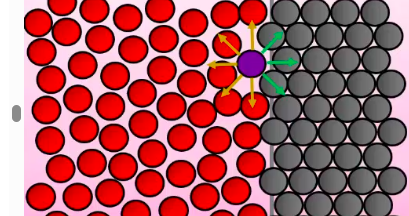
\includegraphics[width=0.75\textwidth]{figures/lec04-05.png}
     \caption{}
\end{figure}


There are two forces in effect here, the interatomic forces of the liquid and of the beaker. We call the forces between the liquid itself cohesion, and between the liquid and a foreign body adhesion.

\subsection{Wetting}
``Wetting'' is the ability of a liquid to maintain contact with a solid surface and is inversely proportional to surface tension. Most liquids are ``wetter'' than water, due to water's high surface tension.

If there are strong adhesive forces, the liquid preferentially sticks to the side of the container, causing the formation of a concave meniscus.

If there are strong cohesive forces, minimisation of surface area causes the formation of a convex meniscus.


\section{Capillary Action}
If an open tube is placed into contact with the surface of a liquid with strong adhesion, the liquid will rise up the sides of the tube:

\begin{figure}[H]
    \centering
    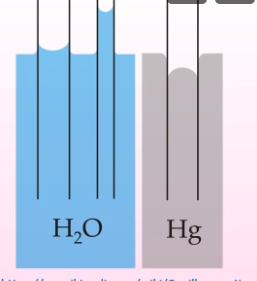
\includegraphics[width=0.5\textwidth]{figures/lec04-06.png}
     \caption{Capillary action for water and mercury. Note that mercury, being strongly cohesive, minimises surface area so does not rise up.}
\end{figure}

We can describe this mathematically in terms of the angle formed by the meniscus, the width of the meniscus and the height reached by the liquid:

\begin{figure}[H]
    \centering
    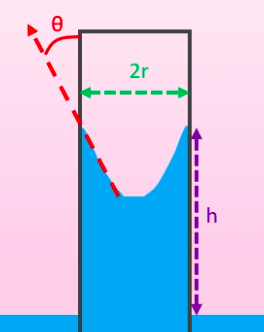
\includegraphics[width=0.4\textwidth]{figures/lec04-07.png}
     \caption{}
\end{figure}

There are two competing forces here:
\begin{itemize}
    \item Surface tension, pulling the liquid up.
    \item The weight of the liquid, pulling it down.
\end{itemize}

The weight is given by the volume (if we approximate the meniscus as being small compared to the total volume, hence just a cylinder) and density:
\[
    F_W = mg = \rho V g =  \rho \pi r^2 h g
\]

Surface tension has units of force divided by length. We can therefore get the force by the multiplying by the active contact length, which is the circumference of the cylinder. Finally, we only care about the vertical component, so take $\cos \theta$:

\[
    F_\gamma = \gamma 2 \pi r \cos \theta
\]

Hence, as equilibrium:
\[
    F_\gamma = F_W
\]

\[
    2 \gamma \pi r \cos \theta = \rho \pi r^2 h g
\]
\[
    2 \gamma \cos \theta = \rho g r h
\]

This gives:
\[
    \boxed{h = \frac{2 \gamma \cos \theta}{\rho g r}}
\]
